\documentclass[a4paper,fontset=fandol]{ctexart}

\usepackage{amsmath,amssymb,amsthm,physics,fancyhdr,geometry,hyperref,graphicx,enumitem,upgreek,booktabs,multirow,longtable}

\geometry{vmargin=2cm,hmargin=2.5cm}

\pagestyle{fancy}
\fancyhf{}
\fancyfoot[C]{\thepage}
\renewcommand{\headrulewidth}{0pt}

\usepackage{titlesec}
\titleformat{\section}
{\normalfont\Large\bfseries}{团队赛\thesection:}{0.5em}{}

\newcommand{\points}[1]{\par % 确保换行
	\noindent % 取消缩进
	\hfill (#1分)% 右对齐并添加分数
	\vspace{1em}
}

%\parskip=1em

\hypersetup{colorlinks}

\begin{document}
	{
	\Large\bfseries\noindent 团队赛:\hspace{0.5em}指导说明
	}
	
	\begin{itemize}
		\item 这一轮中, 参与者将随机选择分为5人团队, 每个团队代表一个命名的小行星. 每个团队中的参与者将来自不同的国家. 分组将在IOAA开始时进行, 以便团队成员可以相互了解. 
		
		\item 请记住你的小行星的名称和编号, 因为这也将在天文馆和观测比赛中用于标识你的位置. 
		
		\item 团队赛包括几个任务, 你将通过一个密封的信封接收它们. 每个团队在向导的监督下在一张桌子上共同解决问题. 在本轮中, 你不得与其他团队的参与者交流. 
		
		\item 提供专用的答题卡用于写下你的答案. 将最终答案填写到答题卡上适当的方框中(标记为A). 
		
		\item 在裁判发出开始信号时打开信封. 从这一刻开始计时: 总用时最短的团队将会获胜, 其中总用时包括罚时(例如, 不正确或缺失的答案). 每个任务中都解释了罚时. 
		
		\item 当你解决了所有问题后, 将你的答题卡交给向导, 他将记录总时间. 
		
		\item 这一轮的最大可用时间是90分钟. 在此之后, 应提交所有剩余的答题卡. 
		
		\item 然后, 评审团将对完成的答题卡进行评分, 并适当应用罚时. 获胜的团队将在闭幕式上宣布. 
		
		\item 桌子上将提供你需要的一切(计算器、办公用品、几何工具、纸张、常数表). 
		
		\item 对于其中一项任务, 房间内的所有屏幕将在指定时间同时显示视频(视频将重复播放几次). 
	\end{itemize}
	
	\newpage
	\section{纵横字谜}
	
	在答题卡的表格中, 每行填写对应符号的国际天文学联合会(IAU)星座三字母缩写. 你最终的答案是通过加粗的垂直列来形成的. 
	
	提示: 下面的星图使用符号标记了Mercator投影法的星座. 
	
	\textbf{罚时: }空白或错误的星座: +1分钟
	
	\begin{center}
		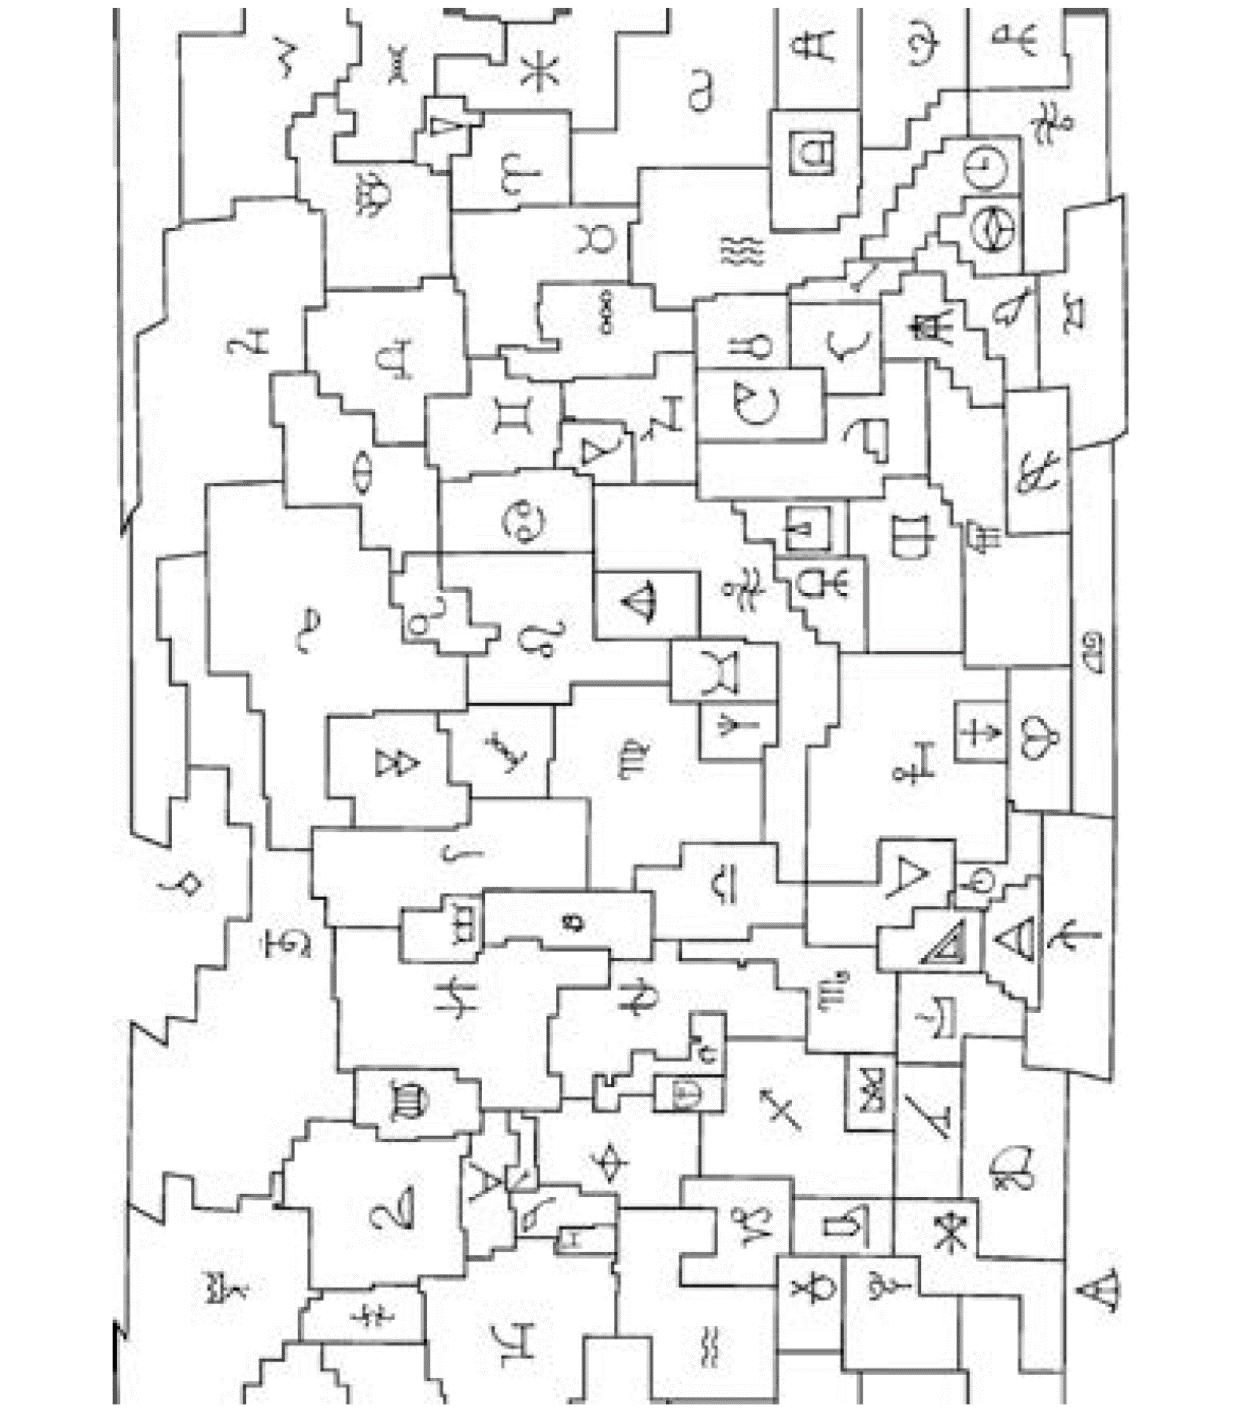
\includegraphics{fig/1.png}
	\end{center}
	
	\begin{center}
		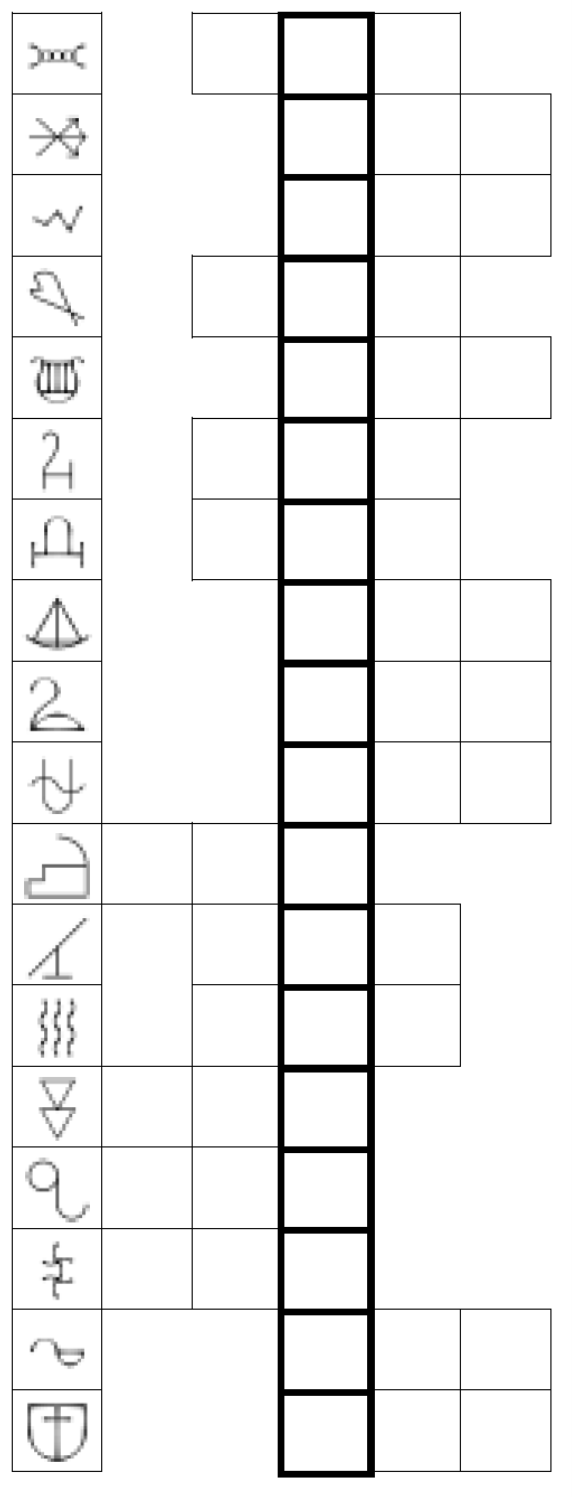
\includegraphics{fig/2.png}
	\end{center}
	
	\newpage
	\section{回复Arecibo信息}\label{2}
	
	在IOAA 2023期间, 1974年由Arecibo射电望远镜发送的信息终于到达了地球. 在比赛期间, 传输的视频记录将在监视器上播放. 解码传输内容并在答题卡上写下隐藏的信息. 
	
	视频将在比赛开始后30分钟开始播放, 并连续循环播放总共30分钟. 
	
	\textbf{罚时: }缺失或错误的答案: +15分钟
	
	\newpage
	\section{火星轨迹}
	
	\begin{enumerate}[label=(\alph*)]
		\item 在提供的坐标纸上, 根据表格中的数据, 绘制地心参考系下地球和火星随时间变化的$X$和$Y$位置, 并在每天绘制连接地球和火星相应位置的矢量. 
		
		\item 使用直尺和三角板, 将每个矢量平移至共同的原点, 同时保持它们的长度和方向. 用一条曲线连接平移后向量的末端, 表示火星在地心参考系中的位置. 
		
		\item 从图表中读取地球与火星之间的最小距离、逆行运动的持续时间以及火星退行的角度. 在答题卡上给出你的答案. 
	\end{enumerate}
	
	\textbf{罚时: }第二部分绘图缺失或错误: +10分钟; 答案缺失或超出范围: 每部分+5分钟. 
	
	\begin{table}[!h]
		\centering
		\begin{tabular}{|l|l|l|l|l|}
			\hline
			\multicolumn{5}{|c|}{日心赤道坐标系位置}\\
			\hline
			&\multicolumn{2}{|l|}{地球}&\multicolumn{2}{|l|}{火星}\\
			\hline
			日期&$X$ [au]&$Y$ [au]&$X$ [au]&$Y$ [au]\\
			\hline
			2022 Sep 01~~~~~~~~ & $0.9375$~~~~~~&$-0.3431$~~~~&$1.3235$~~~~~~&$0.4704$~~~~\\
			2022 Sep 11&$0.9846$&$-0.1928$&$1.2724$&$0.5972$\\
			2022 Sep 21 & $1.0033$ & $-0.0370$ & $1.2082$ & $0.7178$ \\
			2022 Oct 01 & $0.9928$ & $0.1198$ & $1.1320$ & $0.8312$ \\
			2022 Oct 11 & $0.9530$ & $0.2731$ & $1.0448$ & $0.9366$ \\
			\hline
			2022 Oct 21 & $0.8850$ & $0.4184$ & $0.9477$ & $1.0331$ \\
			2022 Oct 31 & $0.7905$ & $0.5512$ & $0.8417$ & $1.1200$ \\
			2022 Nov 10 & $0.6722$ & $0.6673$ & $0.7282$ & $1.1967$ \\
			2022 Nov 20 & $0.5336$ & $0.7631$ & $0.6082$ & $1.2630$ \\
			2022 Nov 30 & $0.3785$ & $0.8356$ & $0.4830$ & $1.3184$ \\
			\hline
			2022 Dec 10 & $0.2119$ & $0.8824$ & $0.3537$ & $1.3628$ \\
			2022 Dec 20 & $0.0387$ & $0.9020$ & $0.2216$ & $1.3960$ \\
			2022 Dec 30 & $-0.1357$ & $0.8936$ & $0.0877$ & $1.4182$ \\
			2023 Jan 09 & $-0.3058$ & $0.8574$ & $-0.0468$ & $1.4294$ \\
			2023 Jan 19 & $-0.4665$ & $0.7947$ & $-0.1810$ & $1.4297$ \\
			\hline
			2023 Jan 29 & $-0.6128$ & $0.7073$ & $-0.3139$ & $1.4194$ \\
			2023 Feb 08 & $-0.7401$ & $0.5981$ & $-0.4445$ & $1.3988$ \\
			2023 Feb 18 & $-0.8447$ & $0.4705$ & $-0.5719$ & $1.3682$ \\
			2023 Feb 28 & $-0.9234$ & $0.3284$ & $-0.6954$ & $1.3280$ \\
			2023 Mar 10 & $-0.9740$ & $0.1765$ & $-0.8140$ & $1.2787$ \\
			\hline
			2023 Mar 20 & $-0.9954$ & $0.0191$ & $-0.9272$ & $1.2207$ \\
			2023 Mar 30 & $-0.9868$ & $-0.1387$ & $-1.0341$ & $1.1545$ \\
			2023 Apr 09 & $-0.9491$ & $-0.2925$ & $-1.1342$ & $1.0807$ \\
			2023 Apr 19 & $-0.8835$ & $0.4377$ & $-1.2268$ & $0.9998$ \\
			2023 Apr 29 & $-0.7920$ & $0.5702$ & $-1.3115$ & $0.9124$ \\
			\hline
		\end{tabular}
	\end{table}
	
	\newpage
	\section{南极星}
	
	在答题卡上的南天球图上, 绘制南天岁差圈, 并确定由于岁差, $\delta$ Velorum(船底座$\delta$星)将成为南极星的年份, 该年份应是最接近现在日期的. 这张地图采用的是等距投影法.
	
	\textbf{罚时: }缺失或错误的答案: +10分钟
	
	\begin{center}
		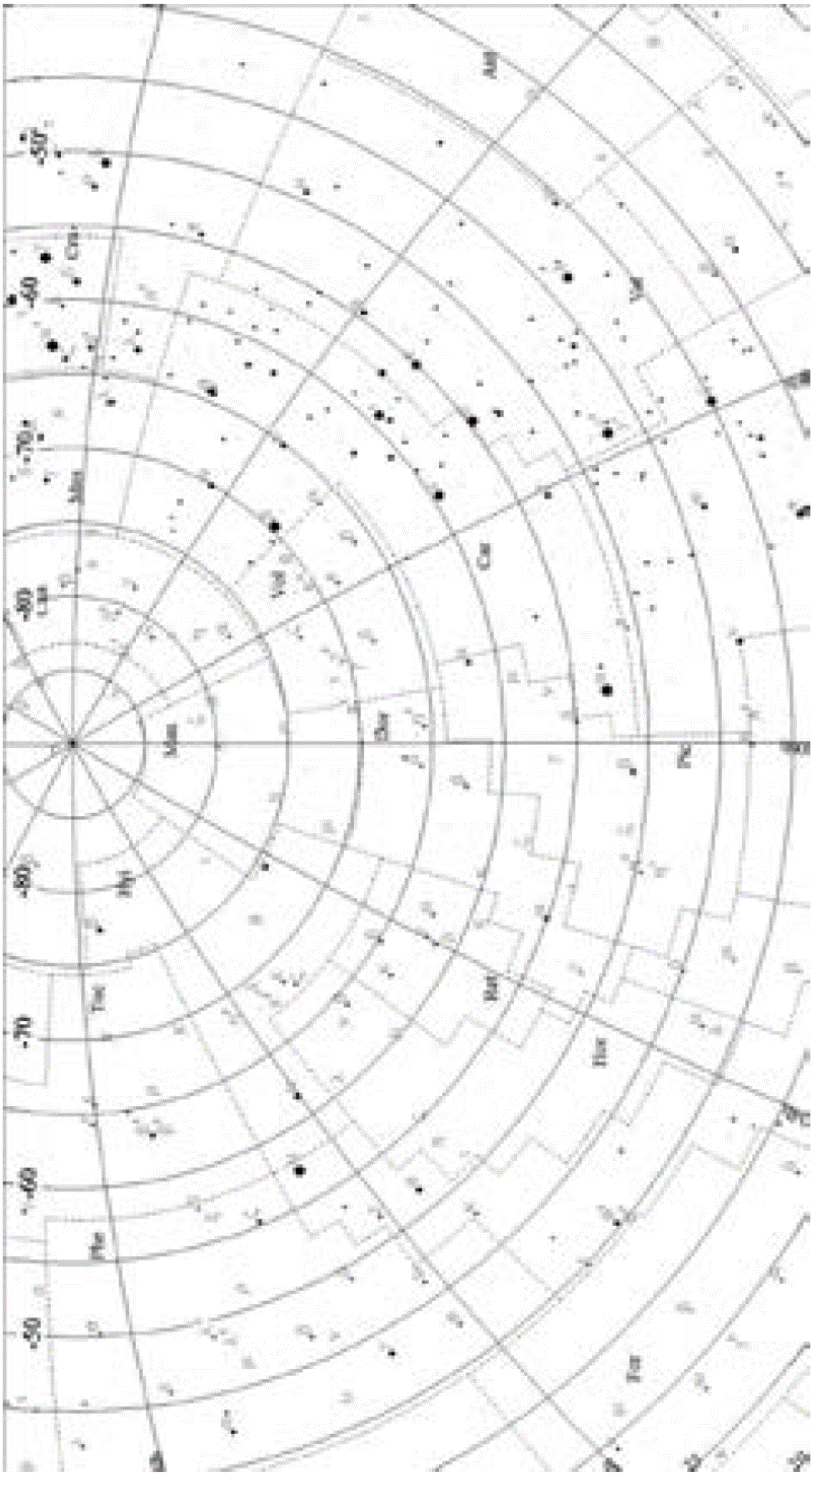
\includegraphics{fig/3.png}
	\end{center}
	
	\newpage
	\section{星盘}
	
	星盘可以帮助你确定选定恒星相对于地平线在给定时间的位置. 基座或称`母盘', 标有地平线、等高度的曲线、极点、回归线、卯酉圈和天赤道(对于纬度$50^\circ\text{N}$). 两个可移动的透明部分是`网板'和`标尺'. `网板'显示了某些恒星的位置, 每个星座各选一个, 就像从天球外部看到的那样, 以及按黄道十二宫划分的黄道. 最后, `标尺'是一个标度, 可以让你确定恒星的赤纬位置. 
	
	\begin{enumerate}[label*=(\alph*)]
		\item 识别网板上用字母标记的恒星, 并在答题卡的表格中完成. 给出名称或Bayer命名法和星座, 以及赤经和赤纬(在$\pm0.25\text{ h}$和$\pm5^\circ$内). 标记出任务\ref{2}中外星传输的源恒星. 
		
		\textbf{罚时: }缺失或错误的名称或错误的坐标: 每个+1分钟; 错误的源恒星+1分钟. 
		
		\item 对于Nicolaus Copernicus的生日(2月19日), 确定太阳的赤经和赤纬(在$\pm0.25\text{ h}$和$\pm5^\circ$内), 以及日出和日落的时间(在$\pm0.25\text{ h}$内). 
		
		\textbf{罚时: }缺失或错误的坐标: +5分钟; 缺失或错误的时间: +5分钟. 
	\end{enumerate}
	
	\begin{center}
		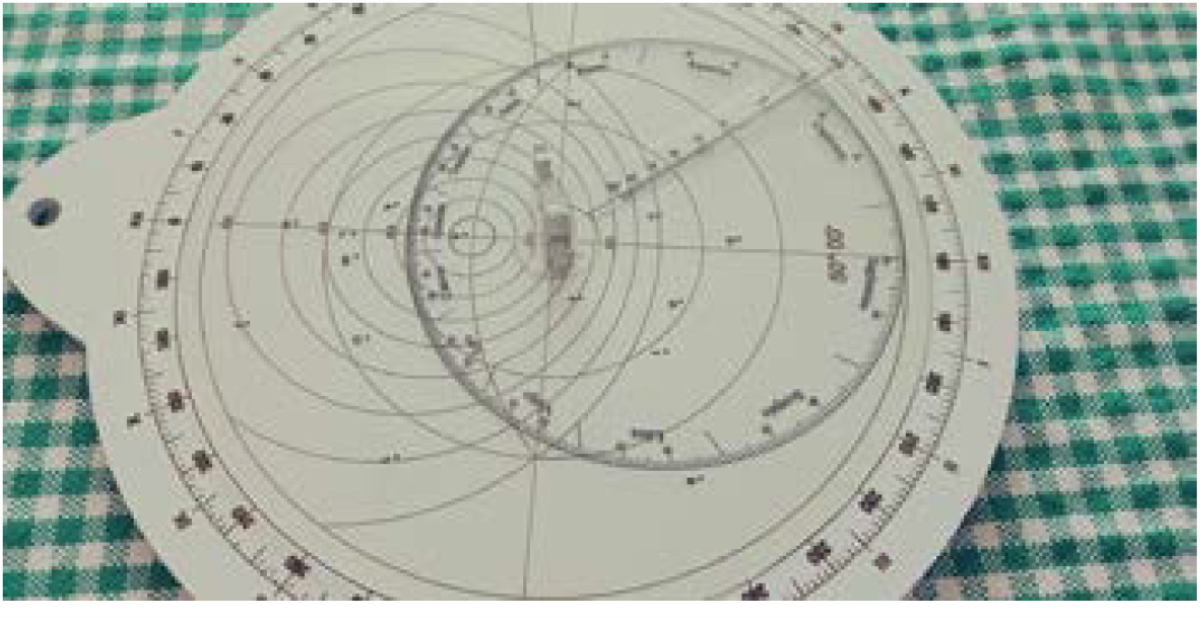
\includegraphics{fig/4.png}
	\end{center}
	
	\newpage
	\section{沙罗周期}
	
	使用过去25年的月食表格来预测下一次从波兰($50^\circ\text{N}$, $19^\circ\text{E}$)可以清晰看到的月食将何时发生. 在答题卡上给出日期和预测的小时. 
	
	\textbf{罚时: }缺少答案+10分钟, 月食可见度弱+1分钟
	
	{\centering
		\begin{longtable}{|l|l|l|l|}
			\hline
			Date & Time UT & Type & JD \\
			\hline
			1991 Dec 21~~~~~~~~ & 10:33:60~~~~~~~~ & Partial~~~~~~~~ & 2448602.940~~~~~~~~ \\
			1992 Jun 15 & 04:57:57 & Partial & 2448788.707 \\
			1992 Dec 09 & 23:45:05 & Total & 2448966.49 \\
			1993 Jun 04 & 13:01:26 & Total & 2449143.042 \\
			1993 Nov 29 & 06:27:06 & Total & 2449320.769 \\
			\hline
			1994 May 25 & 03:31:20 & Partial & 2449497.647 \\
			1995 Apr 15 & 12:19:04 & Partial & 2449823.013 \\
			1996 Apr 04 & 00:10:47 & Total & 2450177.508 \\
			1996 Sep 27 & 02:55:24 & Total & 2450353.622 \\
			1997 Mar 24 & 04:40:28 & Partial & 2450531.694 \\
			\hline
			1997 Sep 16 & 18:47:42 & Total & 2450708.283 \\
			1999 Jul 28 & 11:34:46 & Partial & 2451387.983 \\
			2000 Jan 21 & 04:44:34 & Total & 2451564.698 \\
			2000 Jul 16 & 13:56:39 & Total & 2451742.081 \\
			2001 Jan 09 & 20:21:40 & Total & 2451919.349 \\
			\hline
			2001 Jul 05 & 14:56:23 & Partial & 2452096.115 \\
			2003 May 16 & 03:41:13 & Total & 2452775.653 \\
			2003 Nov 09 & 01:19:38 & Total & 2452952.556 \\
			2004 May 04 & 20:31:17 & Total & 2453130.345 \\
			2004 Oct 28 & 03:05:11 & Total & 2453306.628 \\
			\hline
			2005 Oct 17 & 12:04:27 & Partial & 2453661.003 \\
			2006 Sep 07 & 18:52:25 & Partial & 2453986.286 \\
			2007 Mar 03 & 23:21:59 & Total & 2454163.474 \\
			2007 Aug 28 & 10:38:27 & Total & 2454340.943 \\
			2008 Feb 21 & 03:27:09 & Total & 2454517.644 \\
			\hline
			2008 Aug 16 & 21:11:12 & Partial & 2454695.383 \\
			2009 Dec 31 & 19:23:46 & Partial & 2455197.308 \\
			2010 Jun 26 & 11:39:34 & Partial & 2455373.986 \\
			2010 Dec 21 & 08:18:04 & Total & 2455551.846 \\
			2011 Jun 15 & 20:13:43 & Total & 2455728.343 \\
			\hline
			2011 Dec 10 & 14:32:56 & Total & 2455906.106 \\
			2012 Jun 04 & 11:04:20 & Partial & 2456082.961 \\
			2013 Apr 25 & 20:08:38 & Partial & 2456408.34 \\
			2014 Apr 15 & 07:46:48 & Total & 2456762.824 \\
			2014 Oct 08 & 10:55:44 & Total & 2456938.956 \\
			\hline
			2015 Apr 04 & 12:01:24 & Total & 2457117.001 \\
			2015 Sep 28 & 02:48:17 & Total & 2457293.617 \\
			2017 Aug 07 & 18:21:38 & Partial & 2457983.265 \\
			2018 Jan 31 & 13:31:00 & Total & 2458150.063 \\
			2018 Jul 27 & 20:22:54 & Total & 2458327.349 \\
			\hline
			2019 Jan 21 & 05:13:27 & Total & 2458504.717 \\
			2019 Jul 16 & 21:31:55 & Partial & 2458681.397 \\
			2021 May 26 & 11:19:53 & Total & 2459360.972 \\
			2021 Nov 19 & 09:04:06 & Partial & 2459537.878 \\
			2022 May 16 & 04:12:42 & Total & 2459715.676 \\
			2022 Nov 08 & 11:00:22 & Total & 2459891.958 \\
			\hline
		\end{longtable}
}
	
\end{document}